\section{Propagation atmosphérique et Antennes}
	Les ondes intérragisse avec leur environnement, cela dépend de la fréquence, taille de l'objet rencontré, surface, matériaux, \dots
	
	il existe différente maniere de propagé les ondes:
	\begin{itemize}
		\item onde satellite
		\item onde ionosphère
		\item onde direct
		\item onde de sol
	\end{itemize}
	
	
	\subsection{Ondes direct}
		les ondes sont envoyé en ligne droite a une autre antennes. La porté est limité par l'horizon. Il y a aussi des interférence (distortion/dispersion) avec les onde réfléchie sur le sol.
		
		\begin{figure}[htp]
			\centering
			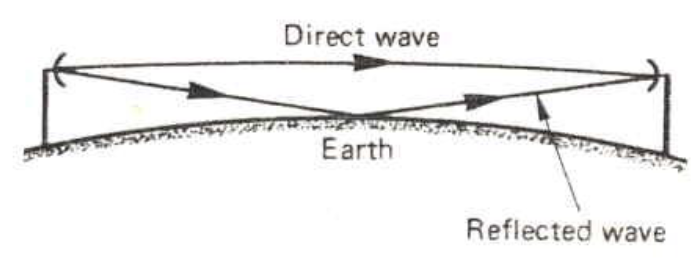
\includegraphics[width=0.7\textwidth]{img/onde_direct.png}
		\end{figure}
	
	\subsection{Ondes de sol}
		Ondes basse fréquences qui se propage généralement le long du sol car le fronts des ondes basses fréquences se déplacement perpendiculairement au sol.
		\begin{center}
			\begin{tabular}{c|c}
			\hline
			Fréquency & Range(Km)\\
			\hline
			100 kHz & 200\\
			1 MHz & 60\\
			10 MHz & 6\\
			100 MHz & 1.5\\
			\hline
		
		\end{tabular}
		\end{center}
		
	\subsection{onde ionosphérique}
		Avec l'effet de l'ionisation de de l'air par les UV du soleil et crée un "mur" contre les ondes et les réfléchie.
		Il y a 4 couches précises de la plus proche a la plus éloignée, $D,E,F_1,F_2$. pendant la nuit il ne reste que une seule couche nommé $F$
		
		\begin{figure}[htp]
			\centering
			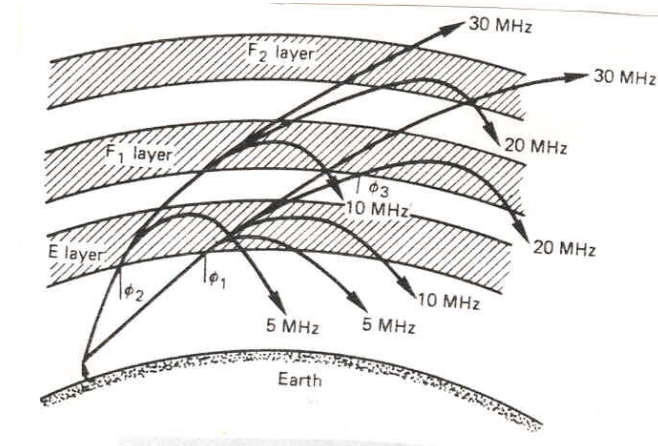
\includegraphics[width=0.7\textwidth]{img/refraction.png}
		\end{figure}
		
		Grace a cela, on peut propager les ondes entre continant. Fort utiliser pour les hondes haute fréquences.
		
		\textbf{MUF} est le Maximal Usable Frenquency, c'est la fréquence max que on est sure a 50\% que elle est réfléchie par la ionosphère.Elle est différente en fonction du jour ou de la nuit.
		
	\subsection{Onde par satellite}
		On a un satellite géostationnaire, qui reste au même endroit par rapport a la terre a qui on envoi le signal et qui le retransmet a d'autre antennes.
		
		\begin{figure}[htp]
			\centering
			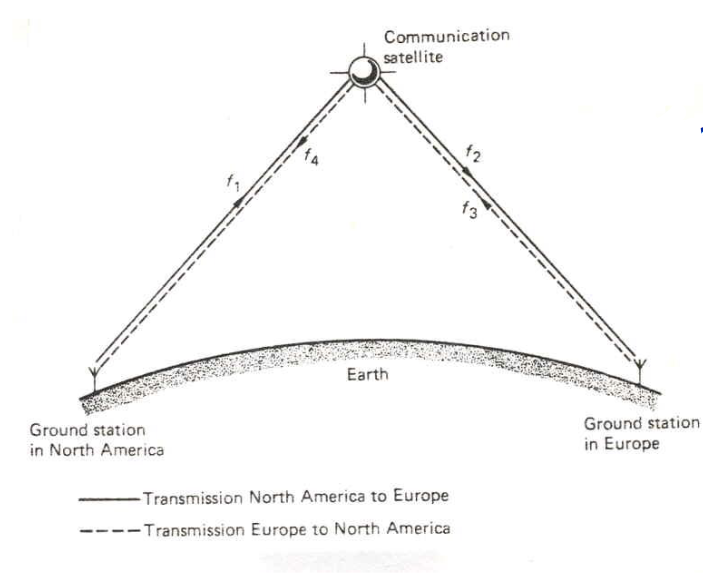
\includegraphics[width=0.7\textwidth]{img/satellite.png}
		\end{figure}
		
	\subsection{Antennes}
		C'est un dispositif qui peut émettre, ou recevoir des ondes électromagnétiques. Autour d'une antennes, on a a des champs magnétique et électrique.
	
		\begin{figure}[htp]
			\centering
			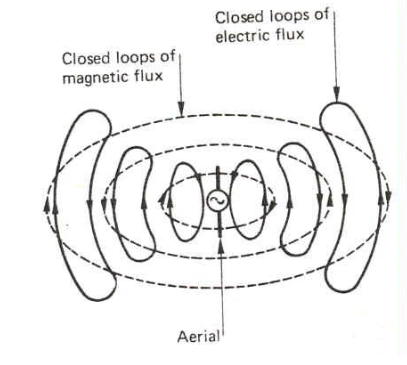
\includegraphics[width=0.35\textwidth]{img/champAntenne.png}
		\end{figure}
		
		\textbf{Onde TEM} (Transverse Electrique-Magnétique), c'est un mode de propagation tel que les champs électrique et magnétique sont tous les 2 orthogonaux a la direction de propagations.
		\begin{figure}[htp]
			\centering
			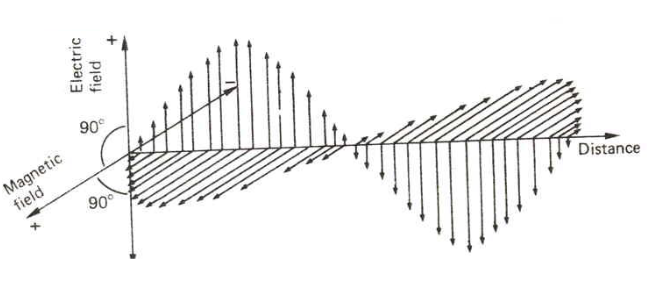
\includegraphics[width=0.45\textwidth]{img/TEM.png}
		\end{figure}
		
		\textbf{Rayonnement} : Quand l'antenne envois une rayonnement dans une direction, elle provoque aussi un rayonnement inverse non désiré. Ce rayonnement a un angle d'ouverture de $\omega$. On peut en mesurer le gains : 
		\begin{equation}
			\text{Gain} = \cfrac{\text{puisasnce dans la direction de puissance max}}{\text{Puissance dans cette direction si l'antenne etais isotrope}}
		\end{equation}
		
		\begin{minipage}{.5\textwidth}
  \centering
  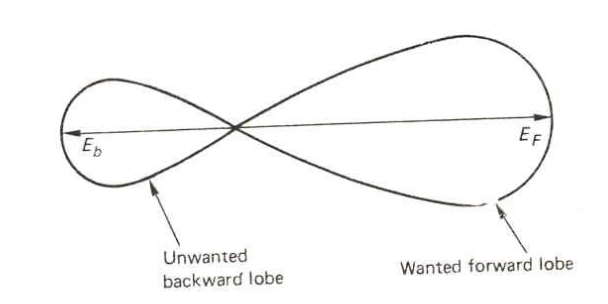
\includegraphics[width=.6\textwidth]{img/rayonnement.png}
\end{minipage}%
\begin{minipage}{.5\textwidth}
  \centering
  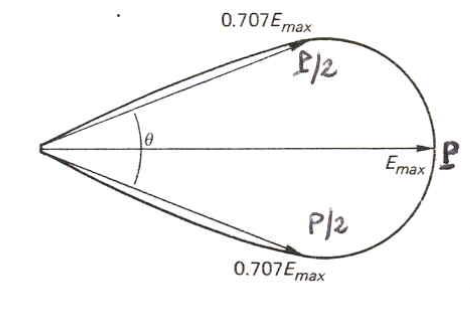
\includegraphics[width=.6\textwidth]{img/rayonnement2.png}
\end{minipage}
\begin{minipage}{.5\textwidth}
  \centering
\end{minipage}

	Il arrive que les ondes envoyé par des antennes, rencontre des objets/obstacle (couche inosphérique, batiment...). Ces objets reflete les ondes et entraine un problème de trajet multiple. C'est un problème qui fait que le meme signal arrive a des moments différents chez le récepteur ce qui entraine des dispersion et de la désynchronisation du signal. On sait que un signal qui varie vite a plus de chance d'avoir un problème de trajet multiple
	
	Il existe différent type d'antennes :
	
	\subsubsection{Dipole $\lambda/2$}
	
		\begin{figure}[htp]
			\centering
			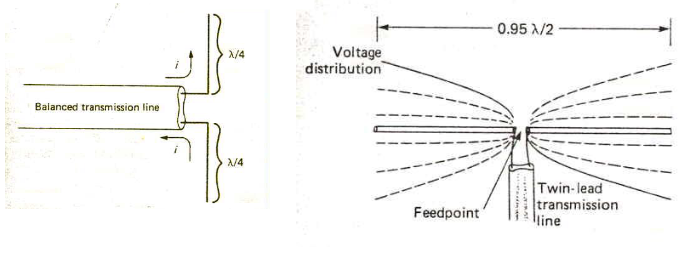
\includegraphics[width=0.7\textwidth]{img/dipole.png}
		\end{figure}
		
		c'est une antenne avec 2 tige de taille $\lambda /4$, les tension au centre sont minime et maximales en extrémité
	
		\begin{minipage}{.6\textwidth}
  \centering
  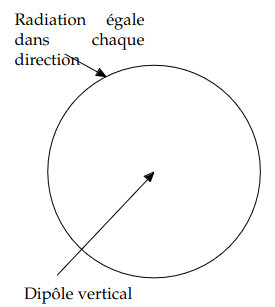
\includegraphics[width=.5\textwidth]{img/dipole1.png}

\end{minipage}%
\begin{minipage}{.5\textwidth}
  \centering
  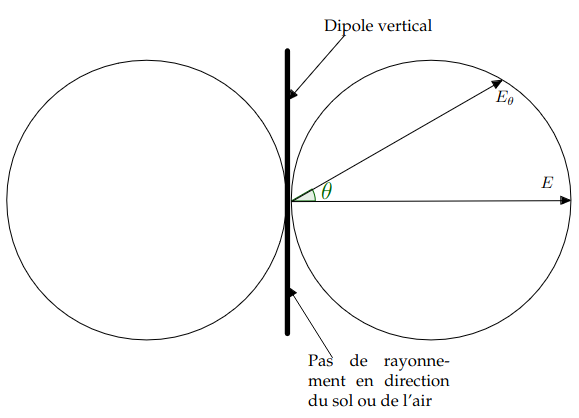
\includegraphics[width=.8\textwidth]{img/dipole2.png}

\end{minipage}
\begin{minipage}{.5\textwidth}
  \centering
\end{minipage}
		On peut minimiser l'antenne avec le principe de miroir qui reflète et simule le signal de l'autre branche.
		
	\subsubsection{Endfire}
		2 dipole de longueur $\lambda/2$ séparé par $\lambda/4$, l'antenne de droite alimente avec une avance de phase de 90° (donc $\lambda/4$) se qui entraine en renforcement vers la gauche
		
		\begin{figure}[htp]
			\centering
			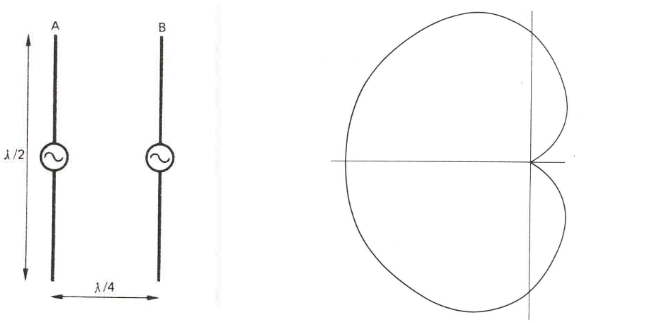
\includegraphics[width=0.6\textwidth]{img/endfire.png}
		\end{figure}
		
	\subsubsection{Yagi}
		Meme principe que les antennes endfire. Composé d'un réflecteur, dipôle et d'un directeur. Antennes très précise car directivité tres étroite. On peut augmenté la directivité en ajoutant des directeur mais diminue la bande passante
		
		\begin{figure}[htp]
			\centering
			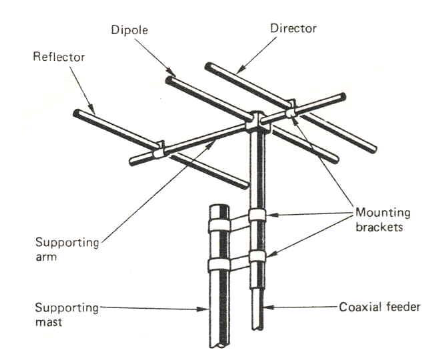
\includegraphics[width=0.35\textwidth]{img/yagi.png}
			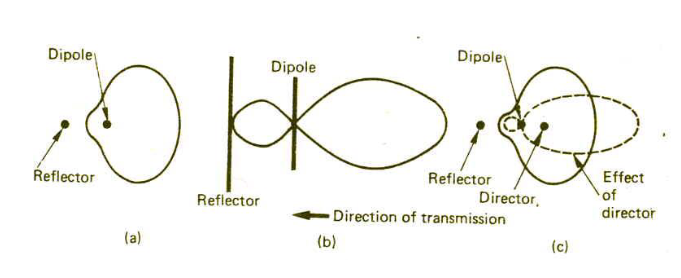
\includegraphics[width=0.55\textwidth]{img/yagi2.png}
		\end{figure}
		
	\subsubsection{Parabolique}
	
		Utilise une parabole pour émettre/recevoir un signal en le point centre de la parabole
		
		\begin{figure}[htp]
			\centering
			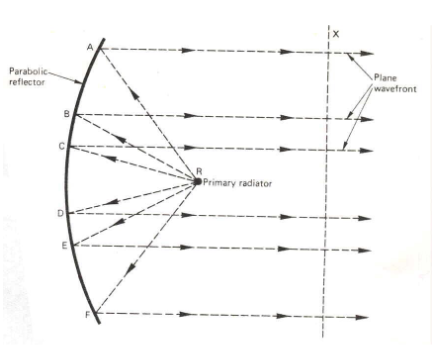
\includegraphics[width=0.45\textwidth]{img/parabole.png}
			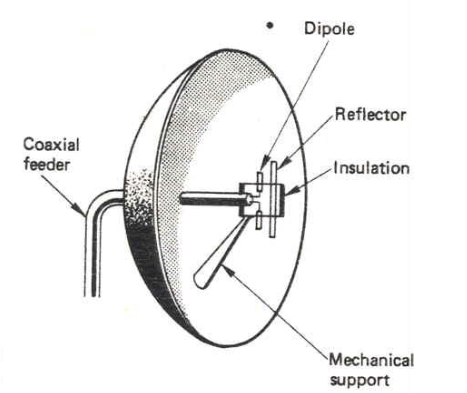
\includegraphics[width=0.45\textwidth]{img/parabole2.png}
		\end{figure}
	\subsubsection{Réseau d'antenne}
		Utilisé pour récuperer un signal faible en "agrégant" des signaux similaire
		\begin{figure}[htp]
			\centering
			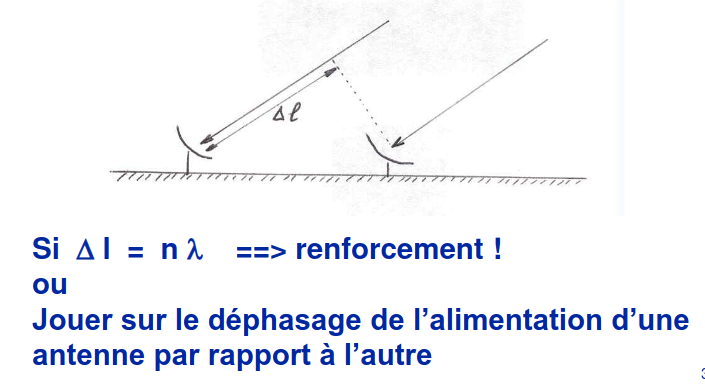
\includegraphics[width=0.7\textwidth]{img/reseauAntennes.png}
		\end{figure}
